\chapter{Engine}

\section{Introduction}

In this chapter, a dataflow engine is presented based on the work detailed in \citet{jennifer_extensible_2017}.
This engine is designed to support parallel execution of instructions by queuing all arguments to instructions and executing these in a scope agnostic way.
Tagged token dataflow is an extension to the data flow model where tags are used to distinguish the execution context of tokens, i.e. multiple calls to the same instruction with different arguments.
For the purposes of this thesis, a lightweight version of this engine has been implemented in Racket to facilitate the mapping process from FrDataFlow. Furthermore, we implemented a mapping layer that translates reactive signals to data flow instructions. Even though there were some mismatches that needed to be addressed, the mapping was successful. 

\newpage
\section{Architecture}

\subsection{Execution of instructions}

Take for example a sample program which computes the average of two numbers, as shown in listing \ref{lst:engine-architecture-sample}

\begin{lstlisting}[caption={Computing the average of two numbers},captionpos=b,label={lst:engine-architecture-sample}]
(define (average x y)
  (/ (+ x y) 2))
  
(average 2 6)
(average 1 5)
\end{lstlisting}

This program computes the average of two numbers twice using different arguments. When this program gets evaluated in the data flow engine, the four arguments are added to the token queue, containing information about which execution context they belong to and what should happen to the result. 
In this example, the 2 and 6 belong to the same execution context, while 1 and 5 will belong to a different one. 

\begin{figure}[h!]
	\includegraphics[width=\textwidth]{images/Engine-Architecture-1.png}
	\caption{The \textit{average} instruction gets called twice}
	\label{fig:engine-architecture-1}
\end{figure}

In figure \ref{fig:engine-architecture-1} we see the arguments queued up against the \textit{average} instruction. Colors indicate the execution context, being positioned lower and more to the left indicates their position in the token queue. At this point, the token queue consists of 2, 6, 1 and 5, wrapped in meta data. 

\begin{figure}[h!]
	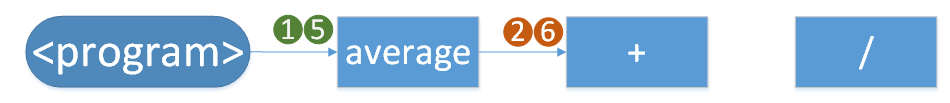
\includegraphics[width=\textwidth]{images/Engine-Architecture-2.png}
	\caption{The arguments are forwarded to the \textit{plus} instruction}
	\label{fig:engine-architecture-2}
\end{figure}

\begin{figure}[h!]
	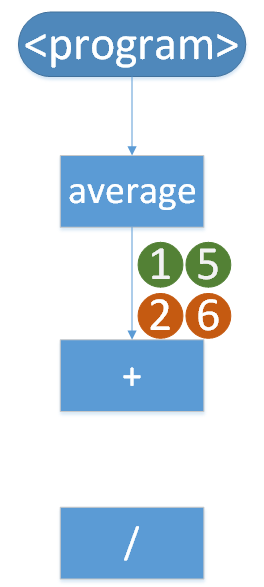
\includegraphics[width=\textwidth]{images/Engine-Architecture-3.png}
	\caption{The next set of arguments are also forwarded to the \textit{plus} instruction}
	\label{fig:engine-architecture-3}
\end{figure}

Since all arguments are present for the first invocation, the \textit{average} instruction gets invoked, as shown in figure \ref{fig:engine-architecture-2}. This calls the plus instruction internally, which adds two new tokens to the queue: 2 and 6.
Because tokens are enqueued at the end, the next thing that happens in figure \ref{fig:engine-architecture-3} is the same step for 1 and 5.

\begin{figure}[h!]
	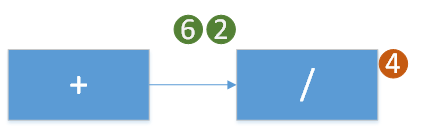
\includegraphics[width=\textwidth]{images/Engine-Architecture-4.png}
	\caption{Results of the \textit{plus} instruction are passed on the \textit{quotient} instruction}
	\label{fig:engine-architecture-4}
\end{figure} 

\begin{figure}[h!]
	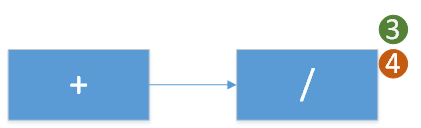
\includegraphics[width=\textwidth]{images/Engine-Architecture-5.png}
	\caption{Results of the second invocation of \textit{plus} are passed on the \textit{quotient} instruction}
	\label{fig:engine-architecture-5}
\end{figure}

When the \textit{plus} instruction has completed its work, it enqueues the result as a new token again, sending it along to the \textit{quotient} instruction. This is possible because of the information contained in the tokens: they know where to go next when instructions have completed. 
In figure \ref{fig:engine-architecture-4} and \ref{fig:engine-architecture-5} we see this process happening for both execution contexts.
Note that the tags are very important here, otherwise the engine would not be aware which arguments belong to the same invocation. There is no guarantee that tokens will always be enqueued in the correct order.

\begin{figure}[h!]
	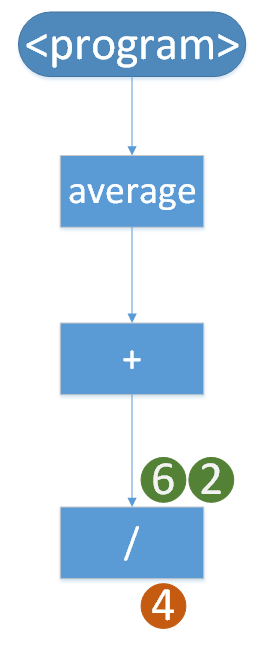
\includegraphics[width=\textwidth]{images/Engine-Architecture-6.png}
	\caption{These results are fed into the quotient operator}
	\label{fig:engine-architecture-6}
\end{figure}

\begin{figure}[h!]
	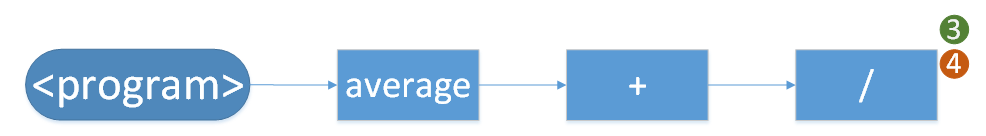
\includegraphics[width=\textwidth]{images/Engine-Architecture-7.png}
	\caption{The second set of results are fed into the quotient operator}
	\label{fig:engine-architecture-7}
\end{figure}

In the end, when the \textit{quotient} instruction has also completed, its results are pushed into the token queue again, as shown by figure \ref{fig:engine-architecture-6} and \ref{fig:engine-architecture-7}. This allows further processing of the data, but is outside the scope of this example. 

To summarize, the general algorithm of the dataflow engine is to process tokens in the queue (FIFO), execute instructions whenever an execution context has all the necessary arguments present and re-enqueue the results of those instructions. Separate invocations are distinguished using tags that denote the execution context.

\section{Mapping of reactive signals to dataflow engine}

To execute our reactive signals on the dataflow engine, a translation step was required to simulate the update loop using the described mechanisms in the dataflow engine.
When we represent reactive programming as a graph, the nodes are signals while the vertices denote dependencies between them.
In the dataflow model, the nodes are instructions and the vertices are data being passed in to them. Therefore, our mapping layers creates data flow nodes for every signal, where the arguments passed in are the parent signal values. When a new value is produced, a token is generated for every child that is subscribed to it.

Taking our example from the Language chapter, we have the following reactive program in figure \ref{fig:engine-mapping-1}.

\begin{figure}[h!]
	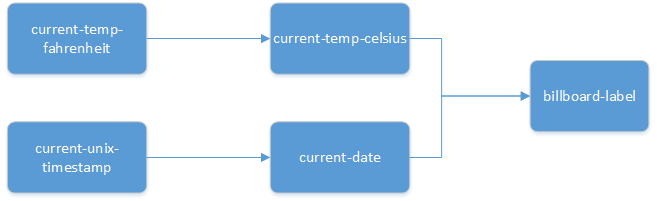
\includegraphics[width=\textwidth]{images/Engine-Mapping-1.png}
	\caption{The billboard program, but the signals are now data flow nodes}
	\label{fig:engine-mapping-1}
\end{figure}

This program behaves exactly the same as the reactive version, the only difference being that is now running atop a dataflow engine.

\subsection{Problems encountered}

\subsubsection{The consumption of arguments in the data flow model}

\paragraph{Problem description}

In reactive programs, signals with a dependency to two or more parent signals are updated whenever at least one of their parents emits a new value. This boils down to the signal functioning as a mapping of the latest values of its parents. Taking our example, this means that when the current temperature changes, the billboard will update immediately, even if the current date has not changed at all.
Similarly, the billboard label updates when the date changes, even if the temperature has not emitted a new value.

In the dataflow engine, an instruction that gets executed consumes its tokens. This is problematic, because when the current temperature emits a new value, it now produces a new token on the queue. 
The billboard label node receives this token, but will keep waiting until the current date produces another token as well. This means that a signal does not update until ALL of its parents have emitted new values.
This was the biggest mismatch between reactive programming and the data flow model, and a perfect solution was not found.

\paragraph{Solution description}

To simulate the same behavior as reactive signals in the data flow model, we had to figure out a way to retrieve the latest values of other parent signals when a new token arrives. 
Although each signal has references to all of its parents, it was not advisable to just read out the latest values and generate extra tokens for the other parents as well. 
This would break our potential for parallelism, because it should be presumed that these dataflow nodes live on and get executed in separate processes and even machines.
The whole premise of the data flow model is that nodes cannot be allowed to access outside state apart from the incoming arguments from the tokens.

The only option that remained was therefore to simulate new signal emissions for all the source signals (signals without parents that get updated by the runtime outside the update loop) whenever one of the source signals emits. Since there is no language support for filtering, throttling or dynamically manipulating the flow of data through the graph, it can be safely assumed that emitting new values from the source signals will ripple through the entire graph, causing all nodes to be updated in the same order. In practice, this meant that whenever a new temperature is sent out, the current second also pushes a value out at the same time. This means the necessary tokens are put on the queue at the same time, simulating the behavior we originally wanted: whenever one parent emits, the other parents do too.

\subsubsection{The evaluation of all instructions in the data flow model}

\paragraph{Problem description}

The data flow engine is actually designed to execute all instructions found in the code, from the highest level abstractions to the lowest primitive operators. The mapping engine was originally designed this way to completely translate not only the signals, but also the statements found in their callbacks to data flow nodes. This meant complete buy-in into the dataflow model, in the hopes of achieving maximum parallelism. However, there is a large mismatch between the traditional Racket language and the dataflow engine: returning values. Whenever a procedure is executed in Racket, it must return a value. In the data flow model, this concept does not exist. Output from instructions is simply enqueued and is not accessible outside the dataflow runtime. Secondly, procedures in Racket carry around with them lexically scoped environments, allowing the use of closures to capture variables or other state that is not enclosed in the body of the procedure definition. 
Again, this violated the core principles of the dataflow engine, which meant we had to scale down the extent to which we made use of the dataflow engine. 

\paragraph{Solution description}

Instead of completely buying into the dataflow engine, we only used its model to implement our reactive signal graph. When parents emit their values, a callback is executed for the signal to update its value. This callback is actually executed inside the interpreter, using the lexical scope assigned to the procedure, without any knowledge or awareness of its presence inside the dataflow engine.
While this has the downside of reduced parallelism, it does improve correctness. Of course, it's impossible to prevent mutating global state or generally causing side effects in these callbacks, but a foolproof mechanism was not the intent of this experiment. 

\section{Conclusion}





